\documentclass[11pt,a4paper]{article}
\usepackage[margin=2.2cm]{geometry}
\usepackage[T1]{fontenc}
\usepackage[expansion=false]{microtype}
\usepackage{booktabs}
\usepackage{tabularx}
\usepackage{array}
\usepackage{enumitem}
\usepackage{xcolor}
\usepackage{listings}
\usepackage{tikz}
\usetikzlibrary{arrows.meta,positioning}
\usepackage{hyperref}
\usepackage{parskip}
\usepackage{amsmath}

\definecolor{accent}{RGB}{0,51,102}
\definecolor{codebg}{RGB}{245,246,248}
\definecolor{boxbg}{RGB}{235,242,250}
\hypersetup{colorlinks=true,linkcolor=accent,urlcolor=accent}

\lstset{
  basicstyle=\ttfamily\small,
  backgroundcolor=\color{codebg},
  frame=single,
  rulecolor=\color{codebg},
  columns=fullflexible,
  keepspaces=true,
  breaklines=true,
  showstringspaces=false,
  tabsize=4,
  xleftmargin=4pt,
  xrightmargin=4pt,
  aboveskip=6pt,
  belowskip=6pt
}

\newcommand{\file}[1]{\texttt{#1}}
\newcommand{\cmd}[1]{\texttt{#1}}
\newcolumntype{L}{>{\raggedright\arraybackslash}X}

\setlist{itemsep=2pt,topsep=4pt}
\setlength{\emergencystretch}{3em}

\title{\color{accent}\textbf{ProEm: Toolchain and Verification Guide}\\[4pt]
\large From SystemVerilog to a Tiny Tapeout chip: simulation, lint, coverage, formal proofs, the ASIC flow and GitHub Actions}
\author{Paul Vincent Bezzina}
\date{17 October 2026}

\begin{document}
\maketitle

\begin{abstract}
This guide explains, from the beginning, every tool and file that takes ProEm from SystemVerilog to a chip, and how to run each check yourself. It assumes you know Verilog from Quartus and ModelSim, but not the open-source ASIC world. Each section explains one idea in general terms, then shows exactly where it appears in the repository. Part~\ref{part:sim} covers simulation, Part~\ref{part:formal} formal verification, Part~\ref{part:asic} the ASIC flow, timing and Tiny Tapeout. The results of running all of it on ISA v0.7.1 are in the verification report (\file{verification\_report.pdf}); this guide is about how the tools work.
\end{abstract}

\tableofcontents
\newpage

%=====================================================================
\part{Getting started}

\section{The big picture}

An FPGA is a chip that already exists; Quartus configures it. An ASIC is a chip that does not exist yet: the tools must decide where every transistor goes and draw the photographic masks a factory uses to make it. The output of that process is a \textbf{GDS file}, a drawing of every layer of the chip.

The journey for ProEm has two branches that meet at the end: one checks the design works (simulation and formal proofs), the other turns it into a layout (the ASIC flow).

\begin{center}
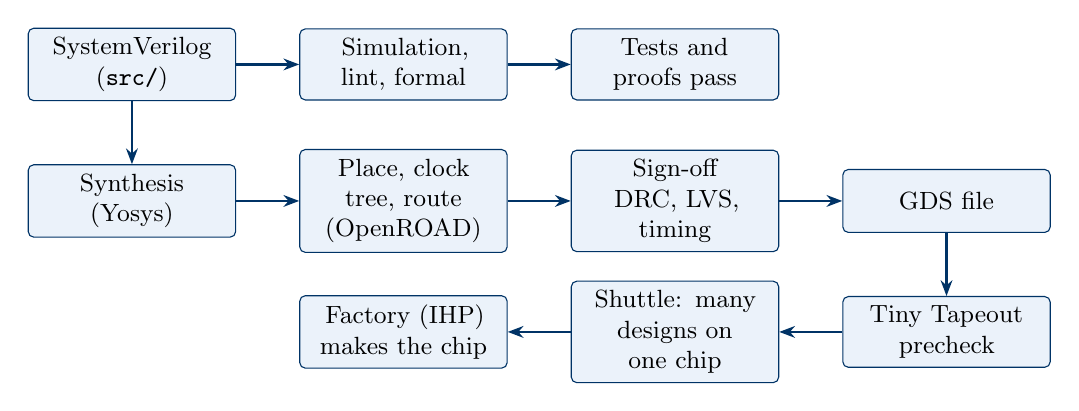
\begin{tikzpicture}[
  box/.style={draw=accent,fill=boxbg,rounded corners=2pt,minimum height=8mm,text width=24mm,align=center,font=\small},
  arr/.style={-{Stealth[length=2mm]},thick,accent}]
\node[box] (rtl) {SystemVerilog\\(\file{src/})};
\node[box,right=8mm of rtl] (sim) {Simulation, lint, formal};
\node[box,right=8mm of sim] (ok) {Tests and proofs pass};
\node[box,below=8mm of rtl] (syn) {Synthesis\\(Yosys)};
\node[box,right=8mm of syn] (pnr) {Place, clock tree, route (OpenROAD)};
\node[box,right=8mm of pnr] (sign) {Sign-off\\DRC, LVS, timing};
\node[box,right=8mm of sign] (gds) {GDS file};
\node[box,below=8mm of gds] (pre) {Tiny Tapeout precheck};
\node[box,left=8mm of pre] (shut) {Shuttle: many designs on one chip};
\node[box,left=8mm of shut] (fab) {Factory (IHP) makes the chip};
\draw[arr] (rtl) -- (sim); \draw[arr] (sim) -- (ok);
\draw[arr] (rtl) -- (syn); \draw[arr] (syn) -- (pnr); \draw[arr] (pnr) -- (sign); \draw[arr] (sign) -- (gds);
\draw[arr] (gds) -- (pre); \draw[arr] (pre) -- (shut); \draw[arr] (shut) -- (fab);
\end{tikzpicture}
\end{center}

Almost all of this runs automatically: when you push to GitHub, \textbf{GitHub Actions} (computers GitHub lends you) run the tests, the proofs and the whole ASIC flow, and show a green tick or a red cross. Your job is to write the SystemVerilog, keep the tests passing, and make sure the \cmd{gds} run is green. Jane Street's instructions say exactly this: start from the CMOS5L template, let the Tiny Tapeout Actions build the GDS and run the precheck, and submit a design with a passing build.

\section{The files in your repository}

\begin{center}
\begin{tabularx}{\linewidth}{@{}lL@{}}
\toprule
File or folder & What it is for \\
\midrule
\file{src/} & The SystemVerilog. \file{top/tt\_um\_vertrex\_star\_proem.sv} is the Tiny Tapeout wrapper; everything else sits under it. \file{src/files.f} lists every source file for the local scripts. \\
\file{src/config.json} & Settings for the ASIC flow (LibreLane): clock period, placement density, timing margins. Section~\ref{sec:json}. \\
\file{info.yaml} & The Tiny Tapeout project description: name, top module, tile size, source files, pin names. Section~\ref{sec:yaml}. \\
\file{test/} & The cocotb tests: \file{test.py}, \file{tb.v}, \file{Makefile}, \file{requirements.txt}. Section~\ref{sec:cocotb}. \\
\file{sim/} & The C++ pin-level test suite: 16 test programs plus the shared \file{bench.h}, and \file{sim/verilator/} which lets the same tests run on Verilator. Section~\ref{sec:cxxrtl}. \\
\file{formal/} & The formal proofs: one harness and one \file{.sby} file per module. Part~\ref{part:formal}. \\
\file{lint/waivers.vlt} & The reviewed Verilator warnings. Section~\ref{sec:lint}. \\
\file{scripts/} & \file{run.sh} (C++ suite), \file{lint.sh}, \file{coverage.sh}, \file{sigrok\_check.py}, \file{formal.sh}, \file{synth\_ihp.sh}, \file{sta.sh}, \file{docs.sh}. \\
\file{.github/workflows/} & What GitHub Actions run on every push: \file{gds.yaml}, \file{test.yaml}, \file{sim.yaml}, \file{formal.yaml}, \file{docs.yaml}. Section~\ref{sec:actions}. \\
\file{docs/} & All documents as PDFs (\file{docs/README.md} lists them) and the datasheet page \file{info.md}; their LaTeX sources are in \file{docs/latex/}, pictures in \file{docs/images/}. \\
\file{gds/} & A copy of the finished layout (GDS, LEF), images, and a results summary. \\
\file{host/} & The Python host library (\file{proem\_host.py}) that builds instruction bytes and decodes replies. \\
\bottomrule
\end{tabularx}
\end{center}

\section{YAML}\label{sec:yaml}

\subsection{What YAML is}

YAML is a plain-text format for writing down structured settings that both people and programs can read. It has only three building blocks:

\begin{itemize}
\item \textbf{A value}: text or a number, such as \texttt{50000000} or \texttt{"6x4"}.
\item \textbf{A map} (also called a dictionary): names paired with values, written \texttt{name: value}.
\item \textbf{A list}: items written one per line, each starting with a dash \texttt{-}.
\end{itemize}

Nesting is shown by \textbf{indentation}, like Python. Everything indented under a line belongs to it.

\begin{lstlisting}
project:              # a map called "project"...
  title: "ProEm"      # ...containing a value called "title"
  tiles: "6x4"
  source_files:       # ...and a list called "source_files"
    - "core/line_codec.sv"
    - "top/protocol_emulator.sv"
\end{lstlisting}

The rules that catch beginners:
\begin{itemize}
\item Indent with \textbf{spaces only}, never tabs. Two spaces per level is the convention.
\item A colon must be followed by a space: \texttt{tiles: "6x4"}, not \texttt{tiles:"6x4"}.
\item \texttt{\#} starts a comment; the rest of the line is ignored.
\item Put text in quotes when it contains a colon, a \texttt{\#}, or starts with a special character. Quoting all text, as \file{info.yaml} does, is the safe habit.
\end{itemize}

\subsection{\file{info.yaml}}

Tiny Tapeout reads this file to learn about the project. The important entries:

\begin{center}
\begin{tabularx}{\linewidth}{@{}lL@{}}
\toprule
Entry & Meaning \\
\midrule
\texttt{title}, \texttt{author}, \texttt{description} & Shown on the Tiny Tapeout website and in the printed datasheet. \\
\texttt{language: "SystemVerilog"} & Tells the tools how to read the sources. \\
\texttt{clock\_hz: 50000000} & The clock wanted on the real chip (50\,MHz). The demo board generates it. \\
\texttt{tiles: "6x4"} & How much of the shared chip ProEm uses: 6 tiles wide, 4 high. This picks the die outline, 1289.28 $\times$ 710.64\,\textmu m. \\
\texttt{top\_module} & The module the flow builds. Must start with \texttt{tt\_um\_} and be unique: \texttt{tt\_um\_vertrex\_star\_proem}. \\
\texttt{source\_files} & Every \file{.sv} file, relative to \file{src/}. A file missing here is invisible to the flow. \\
\texttt{pinout} & Names for each pin, used only for the datasheet and website. It does not change the hardware. \\
\texttt{yaml\_version: 6} & The format version; never change it. \\
\bottomrule
\end{tabularx}
\end{center}

When you add a new SystemVerilog file, add it in \textbf{three} places: \file{info.yaml} (\texttt{source\_files}), \file{test/Makefile} (\texttt{PROJECT\_SOURCES}), and \file{src/files.f} (used by every local script).

The files in \file{.github/workflows/} are YAML too; Section~\ref{sec:actions} explains them.

\section{JSON and \file{src/config.json}}\label{sec:json}

JSON is YAML's stricter cousin: maps are written \texttt{\{ "name": value \}}, lists \texttt{[a, b]}, and every name is in double quotes. JSON has no comments, so the Tiny Tapeout template uses a trick: entries called \texttt{"//"} hold explanatory text, and the tools ignore them.

\file{src/config.json} configures LibreLane, the ASIC flow. The settings that matter:

\begin{center}
\begin{tabularx}{\linewidth}{@{}>{\raggedright\arraybackslash}p{6.2cm}L@{}}
\toprule
Setting & Meaning \\
\midrule
\texttt{CLOCK\_PERIOD: 20} & The clock period in nanoseconds the flow must meet (20\,ns = 50\,MHz). \\
\texttt{PL\_TARGET\_DENSITY\_PCT: 60} & How tightly cells are packed during placement. Higher packs cells closer (shorter wires) but makes routing harder. \\
\texttt{PL\_RESIZER\_HOLD\_SLACK\_MARGIN}, \texttt{GRT\_RESIZER\_HOLD\_SLACK\_MARGIN} & Extra safety the tool adds when fixing hold time (Section~\ref{sec:timing}). \\
\texttt{MAX\_TRANSITION\_CONSTRAINT: 0.75} & Added for ProEm: no signal may take longer than 0.75\,ns to switch (Section~\ref{sec:slew}). \\
\texttt{PL\_RESIZER\_SETUP\_SLACK\_MARGIN: 3.0}, \texttt{GRT\_RESIZER\_SETUP\_SLACK\_MARGIN: 3.0} & Added for ProEm: the resizer aims for 3\,ns of spare setup time rather than just enough, so the slow corner, which the flow does not enforce, passes too. \\
\texttt{RUN\_POST\_GRT\_RESIZER\_TIMING: 1} & Added for ProEm: repair setup again after global routing, when the wire lengths are known. \\
\texttt{FP\_PDN\_VPITCH}, \texttt{FP\_PDN\_VWIDTH} & Spacing and width of the power stripes; set by the CMOS5L template. \\
\bottomrule
\end{tabularx}
\end{center}

Everything below the template's ``DO NOT CHANGE ANYTHING BELOW THIS POINT'' line should be left alone: it matches the Tiny Tapeout chip.

\section{One-time setup (Windows, with WSL)}\label{sec:setup}

Install WSL (Windows Subsystem for Linux) from the Microsoft Store (``Ubuntu''), open the Ubuntu terminal, and install everything the local checks need:

\begin{lstlisting}
sudo apt update
sudo apt install -y iverilog g++ make git python3-pip python3-venv gtkwave verilator sigrok-cli
python3 -m venv ~/proem-env
source ~/proem-env/bin/activate        # run this line again in every new terminal
pip install cocotb==2.0.1 pytest yowasp-yosys
\end{lstlisting}

\texttt{yowasp-yosys} is Yosys packaged for Python, so you do not need to build it. Your Windows folders appear under \file{/mnt/c/}, for example \file{/mnt/c/Users/Paul/Documents/ProEm}. For the formal proofs you also need the OSS CAD Suite (Section~\ref{sec:osscad}).

%=====================================================================
\part{Simulation and checks}\label{part:sim}

\section{Simulation}

\subsection{What a simulator does}

A simulator runs your Verilog on a normal computer so you can check its behaviour before building anything. It keeps a list of events (``clock rises at 20\,ns'', ``this signal changes'') and processes them in time order. You met this in ModelSim. ProEm uses three open-source simulators.

\begin{center}
\begin{tabularx}{\linewidth}{@{}lL@{}}
\toprule
Tool & Role in ProEm \\
\midrule
Yosys CXXRTL & Turns the design into C++ so the 16 pin-level test programs in \file{sim/} run fast. The main regression. \\
Verilator & Lints the code (Section~\ref{sec:lint}), and runs the same C++ tests a second time for coverage (Section~\ref{sec:coverage}). \\
Icarus Verilog & Runs the cocotb tests, on the RTL and on the gate-level netlist. Used by Tiny Tapeout's GitHub Actions. \\
\bottomrule
\end{tabularx}
\end{center}

\subsection{RTL and gate-level simulation}

\begin{itemize}
\item \textbf{RTL simulation} runs the SystemVerilog you wrote. Fast, easy to debug.
\item \textbf{Gate-level (GL) simulation} runs the \textbf{netlist}: the list of real standard cells (AND gates, flip-flops) the flow produced. Each cell comes with a Verilog model from the PDK (\file{sg13cmos5l\_stdcell.v}). It is slower, but it shows the flow did not change the design's behaviour, and it catches things RTL simulation hides, such as a register without a reset starting as \texttt{X}.
\end{itemize}

\subsection{Waveforms}

A waveform file records every signal over time, like ModelSim's wave window. Open it with \textbf{GTKWave} or \textbf{Surfer} (both free). FST is a compressed format; VCD is the older, larger equivalent. The cocotb tests write \file{test/tb.fst}; the C++ tests write a VCD of the pins when asked (Section~\ref{sec:cxxrtl}).

\subsection{Which suite to use}

\begin{center}
\begin{tabularx}{\linewidth}{@{}lLL@{}}
\toprule
 & C++ (CXXRTL) & cocotb (Python, Icarus) \\
\midrule
Speed & Fast: thousands of programs in a minute & Slow: seconds to minutes per test \\
Waveforms & Pins only (\texttt{PROEM\_VCD}) & Every signal, \file{test/tb.fst} \\
Gate-level netlist & No, RTL only & Yes (\texttt{GATES=yes}) \\
Run by GitHub & \cmd{sim} workflow & \cmd{test} and \cmd{gl\_test} jobs \\
Best for & Many scenarios, the standards, random testing, quick checks after every change & Looking inside the design, debugging one scenario, checking the real netlist \\
\bottomrule
\end{tabularx}
\end{center}

A good habit: change the RTL, run the C++ suite (fast), and when something fails and you need to see why, reproduce it in cocotb and look at the waveform.

\section{The C++ test suite (CXXRTL)}\label{sec:cxxrtl}

\subsection{What \file{scripts/run.sh} does}

\begin{enumerate}
\item Yosys reads every file listed in \file{src/files.f} and writes the whole chip as one C++ class into \file{build/emu\_sim.h}. Each port becomes a member: \texttt{rx\_serial} becomes \texttt{p\_rx\_\_serial} (\texttt{p\_} in front, and each underscore doubled).
\item \texttt{g++} compiles each test in \file{sim/} together with that header, producing programs such as \file{build/t\_ps2}.
\item It runs every test with the settings it needs, then (unless \texttt{SKIP\_SYNTH=1}) synthesises the design to report its size.
\end{enumerate}

The tests are pin level: \file{sim/bench.h} sends instruction bytes over the RX pin at a chosen baud rate, decodes what comes back on TX, and lets each test model a real device on the pins (an SPI device, an I\textsuperscript{2}C controller, a USB host). Together they cover the classic protocols, the 16 standards of the standards guide, the CRC and reply, branching, streaming, all four SPI modes, plus 1,800 random programs and 600 random branch programs.

\subsection{Running it}

\begin{lstlisting}
cd /mnt/c/Users/Paul/Documents/ProEm
SKIP_SYNTH=1 bash scripts/run.sh      # all tests, a few minutes
bash scripts/run.sh                    # tests, then synthesis area
\end{lstlisting}
Each check prints a line ending in \texttt{PASS} or \texttt{FAIL} with what was received, and each program ends with \texttt{ALL PASS} or \texttt{FAILED}. The script stops at the first failure.

\paragraph{Run one test again.} After one full run, the programs are in \file{build/}. The number after the name is the setting the test takes; \file{scripts/run.sh} shows the ones it uses:
\begin{lstlisting}
./build/t_ps2 40          # PS/2 with a 40-clock half period
./build/t_spi 6           # SPI with SCK half period 6 clocks
./build/t_random 3 1 150  # seed 3, MSB first, 150 random programs
./build/t_standards dali  # one standard from the standards guide
\end{lstlisting}

\paragraph{Pin waveforms.} Set \texttt{PROEM\_VCD} to write a VCD of the eight protocol pins, the host RX and TX lines and both select outputs:
\begin{lstlisting}
PROEM_VCD=build/dali.vcd ./build/t_standards dali
gtkwave build/dali.vcd
\end{lstlisting}

\paragraph{Rebuild after changing the RTL.} Run \file{scripts/run.sh} again. It regenerates \file{emu\_sim.h} and recompiles everything, which is the simplest way to be sure nothing is stale.

\subsection{The helpers in \file{sim/bench.h}}

\begin{center}
\begin{tabularx}{\linewidth}{@{}>{\raggedright\arraybackslash}p{5.7cm}L@{}}
\toprule
Helper & What it does \\
\midrule
\texttt{power\_on()} & Resets the chip and sends 0x55 for auto-baud. \\
\texttt{CH = 0} or \texttt{1} & Which channel the next instructions address. \\
\texttt{I\_line}, \texttt{I\_clock}, \texttt{I\_start}, \texttt{I\_hdr}, \texttt{I\_main}, \texttt{I\_end}, \texttt{I\_data}, \texttt{I\_branch}, \texttt{I\_run}, and the rest & Build one instruction's bytes, following the ISA. \\
\texttt{cat(\{\ldots\})} & Joins several instructions into one list. \\
\texttt{program(bytes)} & Sends the bytes to the chip over RX and waits until they are delivered. \\
\texttt{idle(n)} & Runs \texttt{n} clock cycles. \\
\texttt{env} and \texttt{pin\_in} & \texttt{env} is a function called every clock cycle; set \texttt{pin\_in} inside it to drive the protocol pins, as a connected device would. \\
\texttt{t.p\_data\_\_out\_\_a.get<bool>()} & Reads a chip output (here channel A's data pin value). \\
\texttt{wait\_return()} & Runs until the chip has finished sending results. \\
\texttt{got[c]}, \texttt{status[c]} & What channel \texttt{c} sent back: data as (bits, value) pairs, and one status byte per frame. \\
\texttt{report(name, ok, detail)} & Prints one \texttt{PASS} or \texttt{FAIL} line. \\
\bottomrule
\end{tabularx}
\end{center}

\subsection{Writing a new test}

This test sends one UART byte (0xA5) into pin 0 and checks that channel A reports it. Save it as \file{sim/t\_my\_uart.cpp}:

\begin{lstlisting}[language=C++]
#include "bench.h"
int line_level = 1;
void my_env() { pin_in = 0xFE | line_level; }   // pin 0 is our UART line

void uart_send(unsigned b, int r) {
  int bits[10]; bits[0] = 0;                     // start bit
  for (int i = 0; i < 8; i++) bits[1 + i] = (b >> i) & 1;
  bits[9] = 1;                                   // stop bit
  for (int i = 0; i < 10; i++) { line_level = bits[i]; idle(r); }
}

int main() {
  env = my_env; power_on();
  int r = 16; CH = 0;
  program(cat({I_line(0, 0), I_clock(ASYNC, r), I_start(0, 1, 0, 0, 0),
               I_main(9, 0), I_run(0)}));
  uart_send(0xA5, r);
  wait_return();
  V exp = {{8, 0xA5}, {1, 1}};
  bool ok = report("UART receive of one byte",
                   got[0] == exp && status[0] == std::vector<unsigned>({1}),
                   show(got[0]) + " |" + showst(status[0]));
  printf(ok ? "ALL PASS\n" : "FAILED\n");
  return !ok;
}
\end{lstlisting}

To compile and run it by itself (after \file{scripts/run.sh} has created \file{build/emu\_sim.h} once):
\begin{lstlisting}
RT=$(python3 -c "import yowasp_yosys,os;print(os.path.join(os.path.dirname(yowasp_yosys.__file__),'share/include/backends/cxxrtl/runtime'))")
g++ -std=c++14 -O2 -I"$RT" -Ibuild sim/t_my_uart.cpp -o build/t_my_uart
./build/t_my_uart
\end{lstlisting}
It prints \texttt{UART receive of one byte ... 8:A5 1:01 | 01 PASS} and \texttt{ALL PASS}. To make it part of the suite, add \texttt{t\_my\_uart} to the \texttt{TESTS} list in \file{scripts/run.sh} (and in \file{scripts/coverage.sh}) and add a line \texttt{./build/t\_my\_uart} with the others.

\paragraph{Random tests and seeds.} \texttt{t\_random} and \texttt{t\_random\_branch} generate random programs from a \textbf{seed} (a starting number for the random generator). The same seed always gives the same programs, so when one fails, rerun it with that seed to reproduce the failure exactly.

\paragraph{Common problems.}
\begin{itemize}
\item \texttt{yosys: command not found}: activate the environment:\\ \texttt{source \textasciitilde/proem-env/bin/activate}.
\item \texttt{emu\_sim.h: No such file}: run \file{scripts/run.sh} once before compiling a test by hand.
\item A test hangs: it is waiting for a reply that never comes. Check the program (wrong channel in \texttt{CH}, missing \texttt{I\_run}) and that \texttt{env} drives the pins the test expects.
\item A new source file is not seen: add it to \file{src/files.f} (and to \file{info.yaml} and \file{test/Makefile}).
\end{itemize}

\section{cocotb}\label{sec:cocotb}

\subsection{What cocotb is}

cocotb (``coroutine co-simulation testbench'') lets you write the testbench in \textbf{Python} instead of Verilog. The simulator (Icarus) runs the hardware; cocotb runs your Python alongside it and can read and drive any signal.

\begin{center}
\begin{tabularx}{\linewidth}{@{}lL@{}}
\toprule
File & Role \\
\midrule
\file{tb.v} & A small Verilog top level that instantiates the chip, adds wiring the tests need (for example, looping channel B's output back to channel A, and an open-drain I\textsuperscript{2}C bus), and starts the waveform dump. \\
\file{test.py} & The six tests: auto-baud and errors, UART loopback, SPI loopback, I\textsuperscript{2}C target loopback, UART at 0x0000, CRC append and check. Each function marked \texttt{@cocotb.test()} is one test. \\
\file{Makefile} & Lists the source files and includes cocotb's own make rules, which call Icarus. \texttt{GATES=yes} switches to the gate-level netlist. \\
\file{requirements.txt} & The Python packages to install (\texttt{cocotb==2.0.1}, \texttt{pytest}). \\
\bottomrule
\end{tabularx}
\end{center}

\subsection{Reading a test}

\begin{lstlisting}[language=Python]
@cocotb.test()
async def test_uart_loopback(dut):
    link = await power_on(dut)          # start clock, reset, send 0x55
    dut.loop_uart.value = 1             # wire B's output into A's input
    ...
    await link.send(program + link.run(0))    # program the chip
    await ClockCycles(dut.clk, 3 * 10 * r + 200)  # let it run
    assert link.got[0] == expected, f"channel A read {link.got[0]}"
\end{lstlisting}

\begin{itemize}
\item \texttt{dut} (``device under test'') is a handle to \file{tb.v}; \texttt{dut.ui\_in.value = 1} drives a pin, \texttt{dut.uo\_out.value} reads one.
\item \texttt{async} and \texttt{await} are how cocotb waits for simulated time. \texttt{await ClockCycles(dut.clk, 100)} pauses the Python until 100 clock edges have passed.
\item \texttt{assert} checks a result; if it is false the test fails and prints the message.
\item The \texttt{Link} class in \file{test.py} turns calls such as \texttt{link.main(9, 0)} into instruction bytes, sends them bit by bit on \texttt{ui\_in[0]}, and decodes the chip's replies from \texttt{uo\_out[0]} into \texttt{link.got} and \texttt{link.status}.
\end{itemize}

\subsection{Running it}

\begin{lstlisting}
cd /mnt/c/Users/Paul/Documents/ProEm/test
make -B                                       # all six tests on the RTL
make -B COCOTB_TEST_FILTER=test_spi_loopback  # one test
gtkwave tb.fst                                # the waveform
\end{lstlisting}

\texttt{-B} forces a rebuild, so the latest RTL is always used. The summary line reads \texttt{TESTS=6 PASS=6 FAIL=0}, and \file{results.xml} is what the GitHub \cmd{test} workflow checks. In GTKWave, expand \texttt{tb} and then \texttt{user\_project} to reach the design's hierarchy (\texttt{core}, \texttt{channel\_a}, and so on). \texttt{uo\_out[0]} is the chip's TX line, \texttt{ui\_in[0]} is RX, and \texttt{uio\_out} and \texttt{uio\_oe} are the protocol pins.

\subsection{Writing a new test}

The same UART check as the C++ example, added to the end of \file{test/test.py}:

\begin{lstlisting}[language=Python]
@cocotb.test()
async def test_my_uart_byte(dut):
    link = await power_on(dut)          # clock, reset, auto-baud
    r = 16                              # 16 clocks per UART bit
    link.channel = 0
    await link.send(link.line(0, 0)     # plain line coding on pin 0
                    + link.clock(ASYNC, r)
                    + link.start(0x00, 1, 0, 0, 0)   # wait for the start bit
                    + link.main(9, 0)   # read 9 bits: 8 data + stop
                    + link.run(0))
    byte = 0xA5
    for level in [0] + [(byte >> i) & 1 for i in range(8)] + [1]:
        dut.ext_in.value = 0xFE | level # pin 0 carries our UART line
        await ClockCycles(dut.clk, r)
    await link.quiet()                  # wait until the chip stops replying
    dut._log.info(f"channel A read {link.got[0]}, status {link.status[0]}")
    assert link.got[0] == [(8, 0xA5), (1, 1)], f"got {link.got[0]}"
    assert link.status[0] == [1], f"status {link.status[0]}"
\end{lstlisting}

Run it with \texttt{make -B COCOTB\_TEST\_FILTER=test\_my\_uart\_byte}. The log shows \texttt{channel A read [(8, 165), (1, 1)], status [1]}: 8 bits with value 165 (0xA5), then the stop bit, then status 0x01 (frame complete). \texttt{dut.ext\_in} is a register in \file{tb.v} that drives the protocol pins from outside, like a device connected to the chip.

\paragraph{Reading internal signals.} Any signal can be read from Python, for example
\begin{lstlisting}
dut.user_project.core.channel_a.chain.base_mode.value
\end{lstlisting} Reading a signal that is \texttt{X} and converting it with \texttt{int(...)} raises ``Can't convert LogicArray to int''. That usually means a register without a reset, or a signal read before reset finished.

\subsection{Gate-level simulation on your computer}

This is optional, because GitHub's \texttt{gl\_test} job does it on every push.
\begin{enumerate}
\item From a green \cmd{gds} run, download the \texttt{tt\_submission} artifact. Inside it, \file{tt\_um\_vertrex\allowbreak\_star\_proem.v} is the routed netlist; copy it into \file{test/} as \file{gate\_level\_netlist.v}.
\item Install the CMOS5L PDK at the revision the CI uses:
\begin{lstlisting}
mkdir ~/pdk && cd ~/pdk && git init -q
git fetch --depth 1 https://github.com/IHP-GmbH/IHP-Open-PDK.git 2bbec755dc67ca3db0261c3d6163e15735d66710
git checkout -q FETCH_HEAD
\end{lstlisting}
\item Install Tiny Tapeout's Icarus 13. Ubuntu's Icarus 12 produces \texttt{X} values with the CMOS5L cell models, so the test fails even though the design is fine:
\begin{lstlisting}
wget https://github.com/TinyTapeout/iverilog/releases/download/v13.0/iverilog_13.0-1_amd64.deb
sudo apt install -y ./iverilog_13.0-1_amd64.deb
\end{lstlisting}
\item Run it: \texttt{cd test \&\& make -B GATES=yes PDK\_ROOT=\$HOME/pdk}. This takes several minutes, because every one of the 25,600 cells is simulated.
\end{enumerate}

\section{Lint}\label{sec:lint}

A \textbf{linter} reads the code without simulating it and reports likely mistakes: width mismatches, signals that are never used, case statements that miss a value, combinational loops. The ASIC flow runs Verilator's linter with the default warnings; \file{scripts/lint.sh} runs it with every warning on (\texttt{-Wall}):

\begin{lstlisting}
bash scripts/lint.sh
lint clean: verilator -Wall, 13 reviewed waivers
\end{lstlisting}

Each warning was read and either fixed or recorded in \file{lint/waivers.vlt} with the file and line it applies to, for example an unused status output the top level does not route. A new warning makes the script fail, so it cannot slip in unnoticed. The \cmd{sim} workflow runs it on every push.

\section{Coverage}\label{sec:coverage}

\textbf{Code coverage} measures which lines and branches of the RTL the tests actually exercise. A line that no test reaches is a line no test checks. \file{scripts/coverage.sh} builds a Verilator model of the design with coverage counters, runs the whole C++ suite on it through \file{sim/verilator/emu\_sim.h} (an adapter that makes the Verilator model look like the CXXRTL one, so the tests are unchanged), merges the counts and annotates the source:

\begin{lstlisting}
bash scripts/coverage.sh
Total coverage (1344/1361) 98.00%
See lines with '%00' in build/cov/annotated
\end{lstlisting}

Search the files in \file{build/cov/annotated/} for \texttt{\%00} to find the points never reached. ProEm's 17 are listed in the verification report: most are \texttt{default} branches that cannot be reached, the rest are corner cases no standard needs. Running the tests on a second simulator is a check in itself: a test that passes on CXXRTL but fails on Verilator points at a race or an uninitialised value.

\section{Independent decode with sigrok}\label{sec:sigrok}

The C++ device models and the RTL were written by the same person, so a misreading of a standard could pass both. \textbf{sigrok} is the open-source logic analyser software, with protocol decoders written independently for each standard. \file{scripts/sigrok\_check.py} records the pins of each standards test as a VCD, decodes it with \cmd{sigrok-cli}, and compares the bytes with values computed separately in Python (CRC-16 Modbus, NMEA checksum, LIN checksum, SMBus PEC):

\begin{lstlisting}
SKIP_SYNTH=1 bash scripts/run.sh       # builds build/t_standards
python3 scripts/sigrok_check.py        # all 30 checks
python3 scripts/sigrok_check.py dali   # one standard
  DALI forward frame (address 03, command 90)    PASS   Raw data: 03 | Raw data: 90
\end{lstlisting}

A failing check prints what the decoder saw. The same decoders run in PulseView against a real logic analyser, so the checks carry over to hardware unchanged.

%=====================================================================
\part{Formal verification}\label{part:formal}

\section{What formal verification is}

A simulation test drives chosen inputs and checks the outputs. However many tests you write, you only learn about the input sequences you tried. 1,800 random programs are a lot, but a FIFO bug that needs ``write, flush, read and write in the same cycle, while full'' may never be generated.

A formal tool works the other way round. You state rules that must always be true (\textbf{assertions}), and the tool searches \emph{every} possible input sequence, mathematically, for one that breaks a rule. Either it proves that none exists, or it hands you the shortest input sequence that breaks it, as a waveform (a \textbf{counterexample}).

\begin{center}
\begin{tabularx}{\linewidth}{@{}lLL@{}}
\toprule
 & Simulation & Formal \\
\midrule
Inputs & The ones your test chooses & All possible inputs, every cycle \\
Answer & ``No failure seen'' & ``Proven'' or ``here is a failing trace'' \\
Best for & Whole-chip behaviour, long protocols & Control logic: FIFOs, pointers, state machines, arbitration \\
Weak at & Rare corner cases & Very large designs, long counters, arithmetic \\
\bottomrule
\end{tabularx}
\end{center}

The two complement each other. ProEm uses simulation for the protocols and the whole chip, and formal proofs for the blocks whose corner cases are hardest to reach by testing. The line codec proof found a real bug (a lost \texttt{tx\_done} after a cancel) that 1,800 random programs had missed.

\section{The tools}\label{sec:osscad}

\begin{center}
\begin{tabularx}{\linewidth}{@{}lL@{}}
\toprule
Tool & Role \\
\midrule
Yosys & Reads the SystemVerilog and the formal harness and turns them into a mathematical model. The same tool does synthesis. \\
SymbiYosys (SBY) & The driver. It reads a small \file{.sby} file, runs Yosys, calls the solver, and reports PASS or FAIL. \\
yices, boolector, bitwuzla, z3 & \textbf{SMT solvers}: programs that answer ``is there any assignment of values that makes this formula true?''. SBY uses them through \file{yosys-smtbmc}. yices is usually the fastest for hardware. \\
ABC (\texttt{pdr}) & A model checker that proves properties with no depth limit by finding an invariant automatically (Section~\ref{sec:modes}). \\
GTKWave or Surfer & Viewers for counterexample and cover waveforms (\file{.vcd}). \\
\bottomrule
\end{tabularx}
\end{center}

The simplest way to get all of them, at matching versions, is the \textbf{OSS CAD Suite}, a single download from YosysHQ. In the Ubuntu (WSL) terminal, open the releases page,\\ \url{https://github.com/YosysHQ/oss-cad-suite-build/releases},\\ copy the link to the newest \file{oss-cad-suite-linux-x64-YYYYMMDD.tgz}, then:
\begin{lstlisting}
cd ~
wget <the link you copied>
tar -xzf oss-cad-suite-linux-x64-*.tgz
source ~/oss-cad-suite/environment    # run this in every new terminal
sby --help                             # check it works
\end{lstlisting}

To make the \texttt{source} line automatic, add it to the end of \file{\textasciitilde/.bashrc}. The \cmd{formal} GitHub workflow installs the same suite with the \texttt{YosysHQ/setup-oss-cad-suite} action.

\section{The four building blocks}

A formal harness is ordinary SystemVerilog plus four kinds of statement.

\paragraph{\texttt{assert}: what must always be true.}
\begin{lstlisting}
assert (full == (count == DEPTH));
\end{lstlisting}
The tool tries to make this false. If it cannot, the property is proven.

\paragraph{\texttt{assume}: what the environment promises.}
\begin{lstlisting}
initial assume (!rst_n);        // the design starts in reset
always_comb assume (ratio != 0); // the divider is never programmed to 0
\end{lstlisting}
Assumptions restrict the inputs the tool may choose. They are powerful and dangerous: an assumption that is too strong can rule out the very case that would fail, and the proof then passes without meaning anything. Keep them few, and only for things the rest of the chip really guarantees.

\paragraph{\texttt{cover}: proof that something can happen.}
\begin{lstlisting}
cover (full);   // show me a trace where the FIFO fills up
\end{lstlisting}
A cover asks the tool to \emph{find} a trace where the condition is true, and writes it as a waveform. Covers catch \textbf{vacuous} proofs: if the FIFO can never become full under your assumptions, every assertion about ``when full'' passes trivially, and the cover exposes that.

\paragraph{Free values: inputs, \texttt{anyconst}, \texttt{anyseq}.}
Every input port of the harness is free: the tool may give it any value in any cycle. For a value that is chosen once and then held, mark a signal \texttt{(* anyconst *)}:
\begin{lstlisting}
(* anyconst *) logic [3:0] ratio;   // any divider from 0 to 15, fixed for the run
\end{lstlisting}
That single line makes the UART proof cover every clocks-per-bit setting at once.

\section{How the tool searches}\label{sec:modes}

\begin{description}[style=nextline,leftmargin=1.5em]
\item[Bounded model checking (\texttt{mode bmc})]
Checks every input sequence up to a fixed length, say 30 cycles from reset. It finds real bugs quickly, but it says nothing about cycle 31, and the work grows quickly with depth.

\item[k-induction (\texttt{mode prove} with \texttt{smtbmc})]
Proves ``if the assertions held for $k$ cycles in a row, they hold in the next one too'' from \emph{any} state, not only reachable ones. It often fails on harmless designs, because the tool starts from impossible states (a harness counter that disagrees with the FIFO's pointers). Fixing this needs extra assertions about internal signals, which a separate harness cannot reach.

\item[PDR, also called IC3 (\texttt{mode prove} with \texttt{abc pdr})]
Builds the missing invariant automatically, by learning which states are unreachable. For control logic like ProEm's buffers and state machines it proves properties with \textbf{no depth limit}. This is what ProEm's proofs use.
\end{description}

Covers always run as a bounded search, since they only need one example.

\section{The harness pattern}

Each proof has two files in \file{formal/}: a harness (\file{\textless module\textgreater\_formal.sv}) and a job description (\file{\textless module\textgreater.sby}). The RTL in \file{src/} is not modified.

\subsection{Why a separate harness}

\begin{itemize}
\item The RTL stays exactly as it is synthesised; nothing is added under \texttt{ifdef}s.
\item The harness only uses the module's ports, so the properties describe the behaviour the rest of the chip relies on, not how the module is built. If you rewrite the module, the same proof still applies.
\item The harness can shrink parameters (a 4-entry buffer instead of 16) to keep the proof fast. The logic is the same for any size.
\end{itemize}

\subsection{A reference model}

The harness keeps a small model of what the module \emph{should} be doing, built only from its inputs and outputs, and asserts that the module agrees with it. For the host FIFO the model is a single counter:

\begin{lstlisting}
assign wrFire = wr_en && !full && !flush;
assign rdFire = rd_en && !empty && !flush;

always_ff @(posedge clk or negedge rst_n) begin
	if (!rst_n) begin
		count <= '0;
	end else if (flush) begin
		count <= '0;
	end else begin
		count <= count + wrFire - rdFire;
	end
end

always_comb begin
	if (started && rst_n) begin
		assert (count <= DEPTH);
		assert (empty == (count == 0));
		assert (full == (count == DEPTH));
	end
end
\end{lstlisting}

\texttt{started} is a flag that is 0 in the very first cycle, so no assertion is checked before reset has been applied.

\subsection{Checking data with one tracked value}

Counting proves the flags, but not that data comes out unchanged and in order. Checking every entry would need a model as large as the FIFO. The standard trick is to follow \emph{one} value, chosen by the tool:

\begin{itemize}
\item A free input \texttt{pick} marks the write the tool wants to follow. The harness records its value and how many entries are ahead of it.
\item Every read moves it one place closer to the front.
\item When it reaches the front, the FIFO's output must equal the recorded value.
\end{itemize}

\begin{lstlisting}
if (!tracking && wrFire && pick) begin
	tracking <= 1'b1;
	trackedValue <= din;
	trackedPos <= count - rdFire;
end
...
if (tracking && trackedPos == 0) begin
	assert (dout == trackedValue);
end
\end{lstlisting}

Because the tool may pick \emph{any} write, with \emph{any} value, at \emph{any} time, proving it for the one tracked value proves it for all of them.

\subsection{The \file{.sby} file}

\begin{lstlisting}
[tasks]
prove
cover

[options]
prove: mode prove
cover: mode cover
cover: depth 30

[engines]
prove: abc pdr
cover: smtbmc yices

[script]
read -formal host_fifo.sv host_fifo_formal.sv
prep -top host_fifo_formal
memory_map

[files]
../src/primitives/host_fifo.sv
host_fifo_formal.sv
\end{lstlisting}

\begin{description}[style=nextline,leftmargin=1.5em]
\item[\texttt{[tasks]}] Two jobs from one file: \texttt{prove} (the assertions) and \texttt{cover} (the covers). A line starting \texttt{prove:} only applies to that task.
\item[\texttt{[options]}] The mode of each task, and the search depth for the cover.
\item[\texttt{[engines]}] PDR for the proof, and yices through \texttt{smtbmc} for the covers.
\item[\texttt{[script]}] The Yosys commands. \texttt{read -formal} enables \texttt{assert}, \texttt{assume} and \texttt{cover}. \texttt{prep -top} picks the harness as the top module. \texttt{memory\_map} turns the FIFO's storage array into ordinary registers, which the solvers handle much faster.
\item[\texttt{[files]}] The files SBY copies into its work folder.
\end{description}

SBY also converts asynchronous resets for you, so \texttt{always\_ff @(posedge clk or negedge rst\_n)} needs no special handling.

\section{Running proofs and reading the results}

\begin{lstlisting}
bash scripts/formal.sh              # all proofs
cd formal && sby -f host_fifo.sby   # one proof, both tasks
sby -f host_fifo.sby prove          # one task only
\end{lstlisting}

\file{scripts/formal.sh} prints one line per module:

\begin{lstlisting}
PASS  branch_unit (prove and cover)
PASS  crc_unit (prove and cover)
PASS  frame_buffer (prove and cover)
PASS  host_fifo (prove and cover)
PASS  line_codec (prove and cover)
PASS  uart_tx (prove and cover)
\end{lstlisting}

Each task writes a folder such as \file{formal/host\_fifo\_prove/}. The last lines of its \file{logfile.txt} say \texttt{DONE (PASS, rc=0)} or \texttt{DONE (FAIL, rc=2)}.

\subsection{When a proof fails}

The log names the failing assertion by file and line, and the folder holds a counterexample:
\begin{lstlisting}
Assert failed in frame_buffer_formal: frame_buffer_formal.sv:113 ...
counterexample trace: frame_buffer_prove/engine_0/trace.vcd
\end{lstlisting}
Open \file{trace.vcd} in GTKWave. It is the shortest input sequence, from reset, that breaks the assertion. Read it like a failing simulation: find the cycle where the assertion fails, then walk back to see which input caused it. Then decide whether the RTL is wrong, or the property or an assumption is.

\subsection{Checking that a proof has teeth}

A proof that cannot fail is worthless, so plant a bug on purpose, on a copy of the RTL, and confirm the proof catches it:

\begin{center}
\begin{tabularx}{\linewidth}{@{}LL@{}}
\toprule
Planted bug & Result \\
\midrule
Frame buffer: rollback restores the write pointer to \texttt{cm\_ptr + 1} instead of \texttt{cm\_ptr} & FAIL at once, with a trace \\
Branch unit: rule 1 given priority over rule 0 & FAIL at once, with a trace \\
CRC unit: the chunk loop takes one bit more than \texttt{feed\_len} & FAIL at once, with a trace \\
\bottomrule
\end{tabularx}
\end{center}

Covers do the same job in the other direction: each cover must be \emph{reached}, or the property it guards may be vacuous.

\section{The six ProEm proofs}

All are unbounded (PDR). Most take a few seconds; the line codec takes about 20\,s and the CRC unit about four minutes.

\subsection{Host FIFO (\file{host\_fifo\_formal.sv})}
Occupancy never exceeds the depth; \texttt{full} and \texttt{empty} match the count exactly; \texttt{flush} empties it; any value written comes out unchanged and in order. Covers: the FIFO fills; a tracked value travels the whole depth.

\subsection{Frame buffer (\file{frame\_buffer\_formal.sv})}
The model keeps two counts: entries written and not yet read (\texttt{total}), and entries committed and not yet read (\texttt{committed}). It proves:
\begin{itemize}
\item \texttt{committed} $\le$ \texttt{total} $\le$ depth, and \texttt{full}, \texttt{almost\_full} and \texttt{empty} are exact (\texttt{empty} is based on committed entries only, so the reader never sees a half-built frame);
\item rollback discards exactly the uncommitted entries (a tracked value that was not yet committed is dropped; a committed one survives);
\item \texttt{commit\_all} includes a write in the same cycle;
\item a tracked value appears on \texttt{dout} the cycle after it is read (the output is registered). The memory write is delayed by one clock with a bypass on the read side; the proof covers that too, since it only looks at the ports.
\end{itemize}

\subsection{UART transmitter (\file{uart\_tx\_formal.sv})}
With \texttt{ratio} free (\texttt{anyconst}, 1 to 15), the model counts bits and cycles, and the proof shows every frame is a start bit, eight data bits LSB first and a stop bit, each held for exactly \texttt{ratio} clocks; the line is high whenever idle; and \texttt{tx\_ready} is high exactly when idle. Cover: a full frame of 0xA5 at 3 clocks per bit.

\subsection{Branch unit (\file{branch\_unit\_formal.sv})}
The harness models the two BRANCH rules from the ISA, loaded through the same configuration writes: compare the chosen block's byte under the mask with the value; take the hit or miss action; for a read-back rule, fire on a mismatch; rule 0 wins over rule 1; each rule acts at most once per frame, until the next frame starts or the rule is rewritten. It proves that \texttt{set\_mode} and \texttt{new\_mode} give the chosen action in the same cycle and only inside a frame; that \texttt{hit} and \texttt{branch\_abort} follow one cycle later and are suppressed by a frame reset; that \texttt{stall} is high for exactly the decision cycle and the abort cycle; and that \texttt{line\_watch} is set exactly when a read-back rule is enabled. A rule with \texttt{SRC} = 1 and \texttt{BLOCK} = 1 fires on the CRC result event and takes its hit action exactly when the CRC was good. The branch unit reference (\file{branch\_unit.pdf}) explains the module itself.

\subsection{CRC unit (\file{crc\_unit\_formal.sv})}
The chip keeps the CRC register top aligned in 16 bits and updates it with up to 8 bits per clock. The harness keeps a second, textbook model: a register of exactly the configured width, right aligned, updated one bit at a time with the polynomial masked to that width. Width, polynomial, initial value, residue, inversion and every input are free, so the proof covers every CRC of 1 to 16 bits. It proves:
\begin{itemize}
\item the chip's register is always the model shifted to the top (\texttt{crc\_out}, inverted when asked);
\item \texttt{good} is exactly ``model equals residue'';
\item feeding the register its own value, top bit first, always leaves zero. This is why a CRC appended without inversion checks with residue 0 at the receiver;
\item the configuration outputs (\texttt{enabled}, \texttt{check}, \texttt{append}, \texttt{width}, \texttt{cover\_from}) match the last configuration write.
\end{itemize}
The assertions are skipped for the cycle after a configuration write, while the register reloads. Covers: a 16-bit CRC good after three chunks; a 5-bit CRC with the USB residue \texttt{0x0C}; an inverted output of all ones.

\subsection{Line codec (\file{line\_codec\_formal.sv})}
The harness counts entries the codec has accepted and not yet answered, and leaves every line, clock and output configuration free and allowed to change at any time. It proves:
\begin{itemize}
\item \texttt{tx\_done} never pulses with nothing outstanding, and at most four entries are ever outstanding;
\item once the select output has been inactive for three clocks, every accepted entry has had exactly one \texttt{tx\_done}, including entries dropped by any pattern of cancels;
\item with \texttt{DRIVE} = \texttt{00} no output enable is ever set; with open drain the data and clock outputs only pull low; the clock output is only enabled while the codec generates the clock.
\end{itemize}
Covers: a cancel with two entries outstanding, a Manchester entry and an I\textsuperscript{2}C entry. The script flattens the design and adds \texttt{setundef -anyseq} (see Pitfalls). The line codec reference (\file{line\_codec.pdf}) explains the module.

\section{Pitfalls}

\begin{description}[style=nextline,leftmargin=1.5em]
\item[Too-strong assumptions] An assumption that removes real inputs makes a proof meaningless. Every assumption should describe something the surrounding logic truly guarantees. Covers help catch this.
\item[Checking during reset] Guard assertions with \texttt{started \&\& rst\_n}, or the tool will ``fail'' on the first cycle before reset has taken effect.
\item[Memories] Arrays make the solvers slow or fail; \texttt{memory\_map} in the script fixes this for small arrays.
\item[Large parameters] Proof time grows quickly with widths and depths. Shrink parameters in the harness when the logic does not depend on them.
\item[Long counters] A 16-bit baud counter has 65,536 states per bit. Constrain the value range, or shrink the counter width in the harness, as the UART proof does with a 4-bit ratio.
\item[Undefined bits] Reading past the end of a vector gives \texttt{x} bits, and newer Yosys versions refuse them with ``Design contains 'x' or 'z' bits''. Pad vectors in the harness, and where the RTL itself does this behind a guard, add \texttt{setundef -anyseq} to the script, as \file{branch\_unit.sby} and \file{line\_codec.sby} do. \texttt{-anyseq} lets the bits take any value in every cycle, so the proof must hold whatever they are.
\item[Solver differences] If one engine is slow, try another: \texttt{abc pdr} for unbounded proofs, \texttt{smtbmc yices} for bounded proofs and covers.
\end{description}

Not yet proven, and checked by simulation instead: the UART receiver (the auto-baud measurement makes the state space large), the bit counters of the frame chain, the bit-level timing of the line codec, and the control unit.

%=====================================================================
\part{From RTL to chip}\label{part:asic}

\section{The ASIC flow (LibreLane)}

\textbf{LibreLane} (the successor of OpenLane) is a script that runs about 80 steps in order, calling several open-source programs. Each step's output is in \file{runs/wokwi/NN-step-name/}. The main stages, with ProEm's numbers from the v0.7.1 layout:

\subsection{1. Lint and synthesis (Verilator, Yosys)}

Verilator checks the code. Then \textbf{Yosys} performs \textbf{synthesis}: it turns the RTL into a netlist of \textbf{standard cells}, the pre-designed gates the factory offers (for example \texttt{sg13cmos5l\_nand2\_1}: a 2-input NAND, drive strength 1). This is what Quartus's ``Analysis and Synthesis'' does for LUTs; here the building blocks are real gates. ProEm becomes about 19,000 cells. \file{scripts/synth\_ihp.sh} runs the same mapping locally, to compare the size of two versions of the RTL without running the whole flow.

\subsection{2. Floorplan and power grid}

The flow creates the empty die (6 $\times$ 4 tiles), places the pins where Tiny Tapeout expects them, draws rows for cells to sit in, and lays a \textbf{power distribution network} (PDN): metal stripes carrying the supply (VPWR, 1.2\,V) and ground (VGND) to every row. These are the regular vertical stripes in the layout pictures.

\subsection{3. Placement (OpenROAD)}

Every cell gets a position. Global placement spreads cells to keep connected ones close; detailed placement snaps them into legal row positions without overlap.

\subsection{4. Clock tree synthesis (CTS)}

ProEm's 2,763 flip-flops all need the clock at nearly the same moment. CTS builds a tree of buffers (362 cells) so the clock arrives everywhere with little \textbf{skew} (difference in arrival time).

\subsection{5. Resizing and timing repair}

The \textbf{resizer} swaps cells for stronger or weaker versions and inserts buffers to fix timing. On ProEm it adds about 6,100 repair buffers: delay cells (\texttt{dlygate4sd3}) to fix \textbf{hold} time, and buffers that split long, heavily loaded wires to fix \textbf{setup} time. This is why the cell count grows from about 19,000 to about 25,600.

\subsection{6. Routing}

\textbf{Global routing} plans which region each wire passes through; \textbf{detailed routing} draws every wire exactly, on the metal layers, obeying the factory's spacing rules. ProEm's wires total about 1.15\,m. The router iterates until there are 0 violations.

\subsection{7. Antenna repair, fill and extraction}

\begin{itemize}
\item \textbf{Antennas}: during manufacturing, a long metal wire connected only to a transistor gate can collect charge and damage it. The flow adds small diodes where needed (51 on ProEm).
\item \textbf{Fill}: empty space is filled with filler and decoupling cells so the chip is uniform to manufacture. Cells cover 43\,\% of the core; the rest is fill, which is why the layout looks full.
\item \textbf{RC extraction}: the flow calculates the real resistance and capacitance of every wire (the \file{.spef} file) so the final timing check uses real wire delays.
\end{itemize}

\subsection{8. Sign-off}

\begin{center}
\begin{tabularx}{\linewidth}{@{}lL@{}}
\toprule
Check & What it proves \\
\midrule
STA (static timing analysis) & Every path meets setup and hold at every corner (Section~\ref{sec:timing}). \\
DRC (design rule check), Magic and KLayout & The drawing obeys every manufacturing rule (minimum widths, spacings, overlaps). A single DRC error can make the chip fail. \\
LVS (layout versus schematic), Netgen & The transistors actually drawn connect exactly as the netlist says. \\
IR drop & The power grid delivers the supply without a large voltage loss (ProEm: 0.23\,mV worst). \\
\bottomrule
\end{tabularx}
\end{center}

\subsection{9. Output}

The final GDS (\file{tt\_um\_vertrex\_star\_proem.gds}) is the drawing sent to the factory. The \textbf{LEF} is a simplified outline with only pin positions, which Tiny Tapeout uses to fit the block into the full chip. A copy of both, with pictures and the full results, is in \file{gds/}.

\section{Timing, explained simply}\label{sec:timing}

\subsection{Setup and hold}

Between two flip-flops sits logic. When the clock ticks, the first flip-flop launches a new value; it travels through the logic and must reach the second flip-flop:
\begin{itemize}
\item \textbf{Setup}: early enough before the \emph{next} clock edge. If the logic is too slow, the second flip-flop captures the old value. A setup failure can be fixed by slowing the clock.
\item \textbf{Hold}: not so early that it overwrites the value being captured at the \emph{same} edge. A hold failure cannot be fixed by slowing the clock, which is why the flow adds delay cells for it.
\end{itemize}

\textbf{Slack} is the spare time. Positive slack means the path passes; negative slack is a violation. The \textbf{maximum clock} is roughly $1 / (\text{period} - \text{setup slack})$: ProEm's slowest path takes $20 - 3.84 = 16.16$\,ns at the slow corner, so about 62\,MHz.

\subsection{Corners}

Real chips vary. Transistors are slower when hot, at low voltage, or when the factory makes them slightly ``slow''. Tools therefore check \textbf{corners} (process, voltage, temperature):

\begin{center}
\begin{tabular}{@{}lllll@{}}
\toprule
Corner & Supply & Temperature & ProEm setup slack & Hold slack \\
\midrule
Slow & 1.08\,V & 125\,$^\circ$C & 3.84\,ns & 0.61\,ns \\
Typical & 1.20\,V & 25\,$^\circ$C & 9.82\,ns & 0.29\,ns \\
Fast & 1.32\,V & $-40\,^\circ$C & 12.35\,ns & 0.10\,ns \\
\bottomrule
\end{tabular}
\end{center}

Setup is hardest at the slow corner; hold is hardest at the fast corner. The CMOS5L flow only \emph{enforces} the typical corner, so a build can be green while failing the slow one. That happened to ProEm twice: in September (fixed with the slew limit below) and after the v0.7.1 additions, when the slow corner missed by 3.8\,ns. The second time was fixed in the RTL, by registering the CRC unit's input and shortening the paths into the frame buffer and the CRC register, plus the larger setup margins in \file{config.json}. The verification report lists each step.

\subsection{Slew}\label{sec:slew}

\textbf{Slew} (or transition time) is how long a signal takes to switch from 0 to 1. A small cell driving a long wire switches slowly, and a slow edge also slows every gate after it. In September ProEm's failing path had edges over 2\,ns long; limiting slew to 0.75\,ns forced the tool to use stronger cells and buffers.

\section{Processes and PDKs}

A \textbf{process} is a factory's recipe for making chips: the transistor size (here 130\,nm, the length of the smallest transistor gate), the number of metal layers for wiring, and the supply voltages. A \textbf{PDK} (process design kit) is the package the factory gives designers: the rules (for DRC), the standard cells with their layouts and timing models (\file{.lib} files), and the Verilog models used in gate-level simulation. IHP, SkyWater and GlobalFoundries publish open PDKs, which is what makes Tiny Tapeout possible.

\begin{center}
\begin{tabularx}{\linewidth}{@{}lL@{}}
\toprule
Process & Notes \\
\midrule
IHP SG13CMOS5L & \textbf{The target for Jane Street.} 130\,nm CMOS from IHP (Germany). Five routing layers: Metal1 to Metal4 plus one thick TopMetal1. Core supply 1.2\,V, I/O 3.3\,V. Cell names start \texttt{sg13cmos5l\_}. \\
IHP SG13G2 & The full IHP 130\,nm process, with seven metal layers and fast bipolar transistors (for radio circuits). Same standard cells, more routing layers. \file{scripts/sta.sh} can use its timing libraries. \\
SkyWater SKY130 & The first open PDK, used by earlier Tiny Tapeout shuttles. \\
GF180 & GlobalFoundries 180\,nm; another Tiny Tapeout option. \\
\bottomrule
\end{tabularx}
\end{center}

Fewer metal layers means fewer ``floors'' for wires, so routing is harder and wires are longer. That is one reason CMOS5L timing is a little slower than SG13G2 for the same design.

\section{How Tiny Tapeout works}

\subsection{Sharing one chip}

Making a chip costs far too much for one small design, so \textbf{Tiny Tapeout} puts hundreds of projects on one die. The die is divided into \textbf{tiles}; each project gets a rectangle of tiles (ProEm: 6 $\times$ 4). A batch of designs manufactured together is a \textbf{shuttle}. After manufacturing (several months), chips are mounted on a \textbf{demo board}. A small microcontroller on the board picks one project at a time through an on-chip multiplexer, supplies its clock and reset, and connects its pins to the board's headers.

\subsection{The pins}

Every project has the same interface, which is why the top module has exactly these ports:

\begin{center}
\begin{tabularx}{\linewidth}{@{}lL@{}}
\toprule
Port & Meaning \\
\midrule
\texttt{ui\_in[7:0]} & 8 inputs. ProEm uses \texttt{ui\_in[0]} as RX from the host. \\
\texttt{uo\_out[7:0]} & 8 outputs. ProEm: TX, BAUD\_LOCKED, ARMED, HOST\_FULL, SELECT. \\
\texttt{uio\_in}, \texttt{uio\_out}, \texttt{uio\_oe} & 8 bidirectional pins. \texttt{uio\_oe[i] = 1} makes pin $i$ an output. ProEm's protocol pins are here, so every line can be driven and read back. \\
\texttt{clk}, \texttt{rst\_n} & Clock, and reset (active low: 0 means reset). \\
\texttt{ena} & 1 when this project is the one selected. \\
\bottomrule
\end{tabularx}
\end{center}

Projects start from Tiny Tapeout's template repository, which contains the workflows, \file{src/config.json}, a sample \file{info.yaml}, and the cocotb test layout. For Jane Street, the template is the \texttt{cmos5l} branch of Tiny Tapeout's IHP template; ProEm matches it.

\section{GitHub Actions: what happens when you push}\label{sec:actions}

\subsection{Workflows}

A \textbf{workflow} is a YAML file in \file{.github/workflows/}. The line \texttt{on: push} means ``run this every time someone pushes''. A workflow has \textbf{jobs}; each job runs on a fresh Linux machine (\texttt{runs-on: ubuntu-24.04}) and has \textbf{steps}. A step either runs a command (\texttt{run:}) or uses a ready-made action (\texttt{uses:}). \texttt{needs: gds} means ``wait for the \texttt{gds} job to finish first''.

\begin{lstlisting}
jobs:
  gds:
    runs-on: ubuntu-24.04
    steps:
      - name: Build GDS
        uses: TinyTapeout/tt-gds-action@ihp-cmos5l   # Tiny Tapeout's action, CMOS5L version
        with:
          pdk: ihp-sg13cmos5l
  precheck:
    needs: gds
    ...
\end{lstlisting}

\subsection{ProEm's workflows}

\begin{center}
\begin{tabularx}{\linewidth}{@{}lL@{}}
\toprule
Workflow and job & What it does \\
\midrule
\cmd{gds} / \texttt{gds} & Installs the CMOS5L PDK and LibreLane, runs the whole ASIC flow, and uploads the results. \textbf{This is the one Jane Street cares about.} \\
\cmd{gds} / \texttt{precheck} & Tiny Tapeout's own checks on the GDS: full KLayout DRC, pins in the right places, right outline, no forbidden layers. \\
\cmd{gds} / \texttt{gl\_test} & Runs the cocotb tests on the routed gate-level netlist the \texttt{gds} job produced. \\
\cmd{gds} / \texttt{viewer} & Publishes a 3D viewer of the layout to GitHub Pages. On a private repository it fails (Pages needs a paid plan), so it is marked \texttt{continue-on-error}. It is not needed for submission. \\
\cmd{test} & The cocotb tests on the RTL. \\
\cmd{sim} / \texttt{simulate} & The C++ test suite, then the sigrok decode of the standards waveforms. \\
\cmd{sim} / \texttt{lint} & \file{scripts/lint.sh}: Verilator with every warning on. \\
\cmd{formal} & Every formal proof (\file{scripts/formal.sh}) with the OSS CAD Suite. \\
\cmd{docs} & Checks \file{docs/info.md} (the datasheet page) can be built. \\
\bottomrule
\end{tabularx}
\end{center}

\subsection{Reading the results}

On GitHub, open the \textbf{Actions} tab. Each push is a row; a green tick means every job passed. Click a run to see each job; click a job to see each step's log; the \texttt{gds} job's summary shows the cell counts, routing statistics and linter output. At the bottom of the run page, \textbf{Artifacts} are downloadable zips:
\begin{itemize}
\item \texttt{tt\_submission}: the GDS, LEF, netlist and settings, the files that go onto the chip.
\item \texttt{GDS\_logs}: every step's reports, for debugging.
\item \texttt{gds\_render}: a picture of the layout.
\end{itemize}

If a job fails, open it and read the last red lines of the failing step. Common causes: a file missing from \file{info.yaml}, a Verilog error the linter reports, or a timing violation at the typical corner. A failure in the upload step (``Artifact storage quota has been hit'') is not a design problem: the account's artifact storage is full. Delete old artifacts or wait for the quota to reset, then press \textbf{Re-run failed jobs} on the run page.

A private repository gets a monthly allowance of free Actions minutes and artifact storage. A full \cmd{gds} run takes tens of minutes, and the precheck DRC can take much longer, so avoid pushing many times in a row just to test small edits; run the local checks first.

\section{Git in five commands}

\begin{center}
\begin{tabularx}{\linewidth}{@{}lL@{}}
\toprule
Command & Meaning \\
\midrule
\cmd{git status} & What has changed since the last commit. \\
\cmd{git add file} & Choose a change to include in the next commit. \cmd{git add -A} includes everything. \\
\cmd{git commit -m "message"} & Save a snapshot with a description. \\
\cmd{git push} & Send the commits to GitHub; this triggers the Actions. \\
\cmd{git log --oneline} & List the commits. \\
\bottomrule
\end{tabularx}
\end{center}

A \textbf{commit} is a snapshot of the whole project. A \textbf{remote} (\texttt{origin}) is the copy on GitHub. A \textbf{tag} (\texttt{v0.7.1}) is a name for one commit. ``Everything up to date'' after \cmd{git push} means there were no new commits to send: you forgot \cmd{git add} and \cmd{git commit}. ``Not a git repository'' means the terminal is not in the folder that contains the hidden \file{.git} folder.

\section{Every check, in one place}

\begin{lstlisting}
bash scripts/lint.sh                     # Verilator -Wall
SKIP_SYNTH=1 bash scripts/run.sh         # every pin-level test (CXXRTL)
cd test && make -B && cd ..              # cocotb, RTL
bash scripts/formal.sh                   # six proofs (OSS CAD Suite)
bash scripts/coverage.sh                 # Verilator coverage, report in build/cov
python3 scripts/sigrok_check.py          # needs sigrok-cli and build/t_standards
PDK_ROOT=~/pdk bash scripts/synth_ihp.sh typ_1p20V_25C   # cell count and area
\end{lstlisting}

Before submitting: push, wait for \cmd{gds}, \texttt{precheck} and \texttt{gl\_test} to go green, and download the \texttt{tt\_submission} artifact.

%=====================================================================
\section*{Glossary}
\addcontentsline{toc}{section}{Glossary}

\begin{description}[style=nextline,leftmargin=1.5em]
\item[ASIC] Application-specific integrated circuit: a chip made for one design, unlike an FPGA.
\item[Assertion] A condition that must hold in every reachable state.
\item[Assumption] A constraint on inputs; the formal tool only considers inputs that satisfy it.
\item[BMC] Bounded model checking: all input sequences up to a fixed depth.
\item[cocotb] Python testbench library that drives a Verilog simulator.
\item[Corner] A combination of process, voltage and temperature at which timing is checked.
\item[Counterexample] A trace, from reset, that breaks an assertion.
\item[Cover] A condition the formal tool must show is reachable.
\item[Coverage] The share of the RTL's lines and branches that the tests exercise.
\item[CTS] Clock tree synthesis: building the buffer tree that distributes the clock.
\item[CXXRTL] Yosys feature that turns Verilog into C++ for fast simulation.
\item[DRC] Design rule check: the layout obeys the factory's geometric rules.
\item[Fill cells] Cells with no logic, placed in empty space for manufacturability.
\item[GDS] The file format of the chip layout sent to the factory.
\item[Gate level] Simulation of the synthesised netlist of real cells rather than the RTL.
\item[GitHub Actions] GitHub's machines that run the workflows on every push.
\item[Harness] A wrapper module that instantiates the design and adds the model and properties.
\item[Hold] Timing check that data does not change too soon after a clock edge.
\item[Icarus Verilog] Open-source Verilog simulator (\cmd{iverilog}, \cmd{vvp}).
\item[Induction] Proving that a property, if true for $k$ cycles, stays true in the next.
\item[Invariant] A property that holds in every reachable state.
\item[LEF] Simplified outline of a block with its pin positions.
\item[LibreLane] The open-source flow that runs synthesis to GDS.
\item[Lint] Automatic check of code for likely mistakes without simulating.
\item[LVS] Layout versus schematic: the drawn circuit matches the netlist.
\item[Netlist] A design described as connected standard cells.
\item[OpenROAD] The program that does floorplanning, placement, CTS, routing and timing.
\item[PDK] Process design kit: rules, cells and models for a manufacturing process.
\item[PDN] Power distribution network: the supply and ground wiring.
\item[PDR / IC3] An algorithm that finds invariants automatically and proves properties without a depth limit.
\item[Precheck] Tiny Tapeout's final checks before a design is accepted.
\item[Reference model] A simple description of the intended behaviour, compared against the design.
\item[RTL] Register-transfer level: the SystemVerilog you write.
\item[SBY] SymbiYosys, the driver that runs Yosys and the solvers from a \file{.sby} file.
\item[Setup] Timing check that data arrives early enough before the clock edge.
\item[Shuttle] A batch of designs manufactured together.
\item[sigrok] Open-source logic analyser software with independent protocol decoders.
\item[Slack] Spare time on a timing path; negative means a violation.
\item[Slew] How long a signal takes to switch.
\item[SMT solver] A program that decides whether a logical formula over bit-vectors can be satisfied.
\item[SPEF] File of extracted wire resistances and capacitances.
\item[Standard cell] A pre-designed gate or flip-flop from the PDK.
\item[STA] Static timing analysis: checking all paths' timing without simulation.
\item[Synthesis] Turning RTL into a netlist of standard cells (Yosys).
\item[Tile] The unit of area on a Tiny Tapeout chip (about 202 $\times$ 155\,\textmu m on IHP).
\item[Utilisation] Share of the core area covered by cells (ProEm: 43\,\% after place and route).
\item[Vacuous proof] A proof that passes only because the situation it talks about can never occur.
\item[Verilator] Open-source Verilog linter and fast simulator.
\item[Workflow] A YAML recipe that GitHub Actions runs.
\item[YAML] Human-readable settings format based on indentation.
\item[Yosys] Open-source synthesis tool.
\end{description}

\end{document}
